\artigotrue
\chapter{TÍTULO DO QUARTO ARTIGO}
\chapternote{Este capítulo é baseado em um artigo que já foi publicado.}
\shorttitle{Quarto artigo}
\label{chap:chapter04}

\begin{chapterabstract}{brazilian}{Palavra-chave 1. Palavra-chave 2. Palavra-chave 3}
Este é o resumo do segundo artigo da tese. Reconheço que este artigo não é muito
diferente do anterior... Mas quem se importa?
\end{chapterabstract}

\begin{chapterabstract}{english}{Key-word 1. Key-word 2. Key-word 3}
This is the abstract of the second article of the thesis. I recognize that it is
not very different from the previous... But who cares?
\end{chapterabstract}

\formatchapter

\section{INTRODUÇÃO}

Este é um capítulo com muitas seções.

\section{FUNDAMENTAÇÃO TEÓRICA}

\blindtext[1]

\section{PROPOSTA METODOLÓGICA}

\blindtext[1]

\section{ÁREA DE ESTUDO}

\section{MATERIAL}

Este também é um texto bem formatado, escrito em Seropédica, RJ. \blindtext[1]

Este é o código fonte de uma função muito complexa construída no ambiente R:

\begin{verbatim}
> soma <- function (a, b) {a + b}
> soma(2, 2)
[1] 4
\end{verbatim}

\section{MÉTODOS}

Está é uma matriz bem formatada, diferente daquelas produzidas pelos editores de
texto tradicionais:

\begin{equation}
  A_{m,n} =
 \begin{pmatrix}
  a_{1,1} & a_{1,2} & \cdots & a_{1,n} \\
  a_{2,1} & a_{2,2} & \cdots & a_{2,n} \\
  \vdots  & \vdots  & \ddots & \vdots  \\
  a_{m,1} & a_{m,2} & \cdots & a_{m,n}
 \end{pmatrix}
\end{equation}

\begin{subequations}\label{eq:maxwell2}
E estas são as equações de Maxwell (sim, de Maxwell!):
\begin{align}
        B'&=-\nabla \times E,\\
        E'&=\nabla \times B - 4\pi j,
\end{align}
\end{subequations}

\section{RESULTADOS}

Para quem ainda não está cansado, aqui está mais um texto bem formatado. 
\blindtext[1]

Que tal fazer um link para a \autoref{fig:ocio2}? E também citar o 
\citeonline{Feyerabend1977} com um link para a localização da referência 
bibliográfica? Sim, isso já foi feito antes!

\begin{figure}[!ht]
\label{fig:ocio2}
\centering
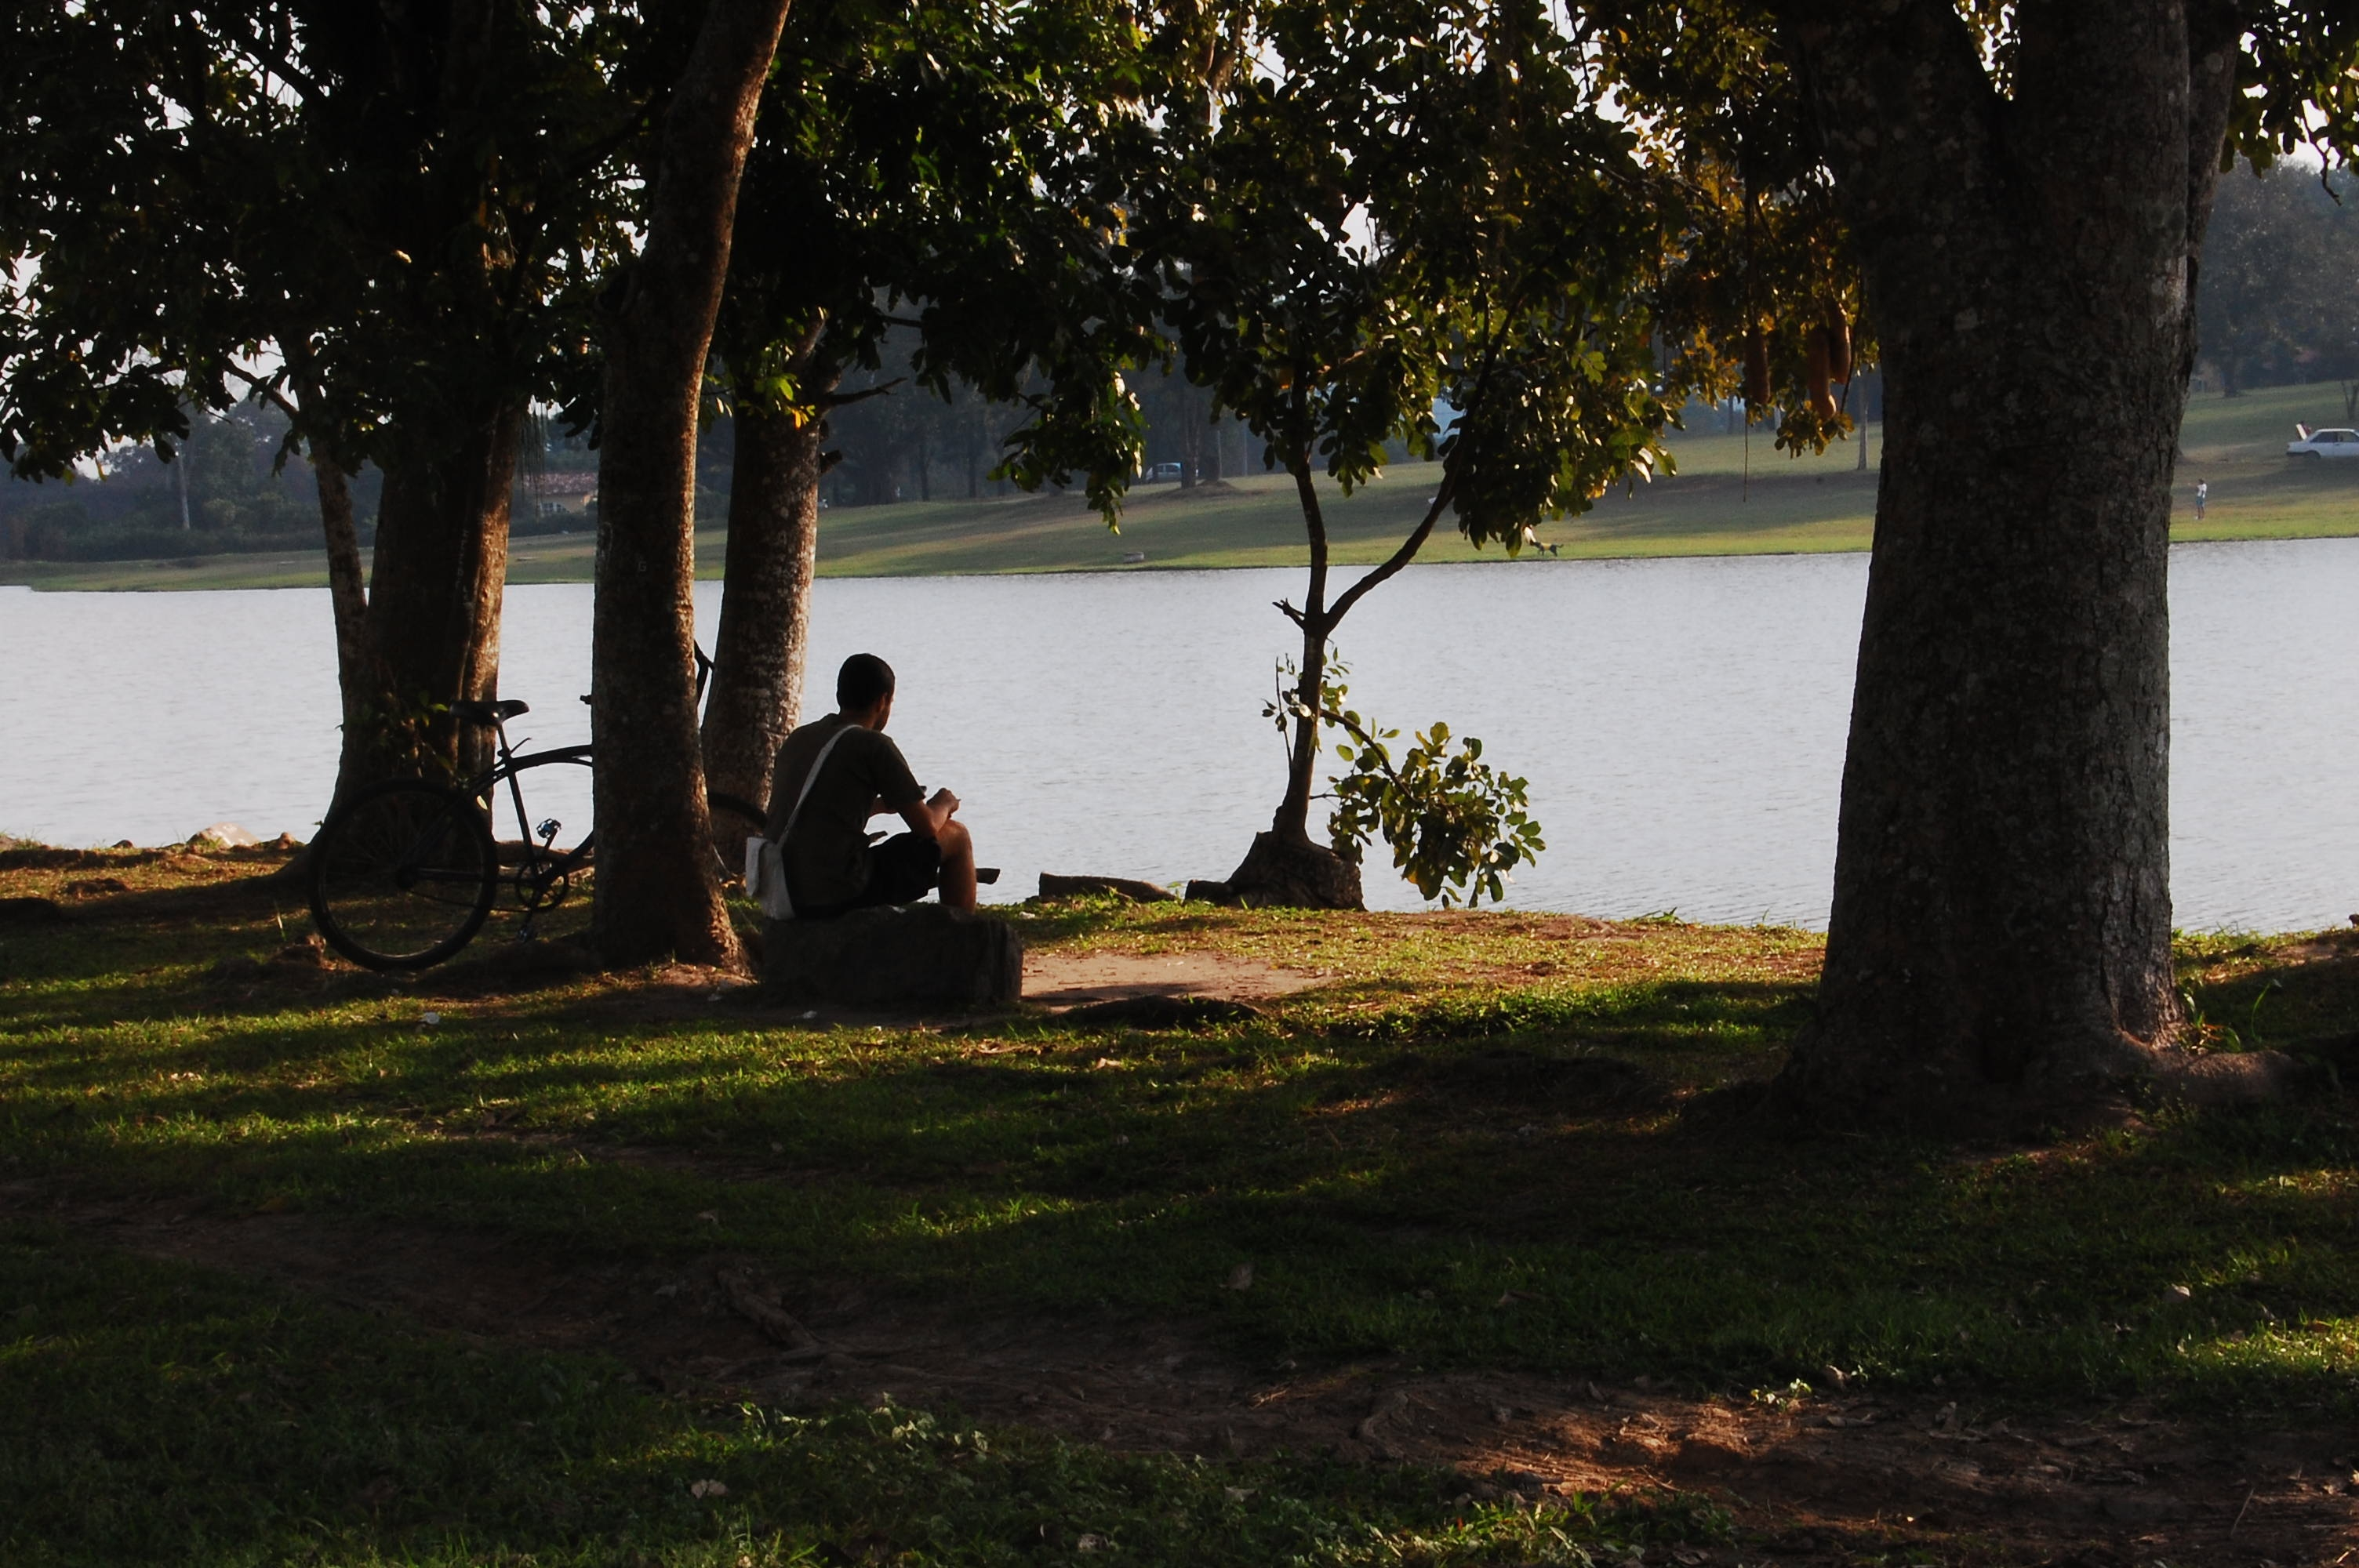
\includegraphics[width=16cm]{figura02}
\caption[O ócio criativo.]{O ócio criativo. Fonte: 
\url{http://r1.ufrrj.br/graduacao/img/acesso-2012/o-ocio-criativo.jpg}}
\end{figure}

\section{DISCUSSÃO}

Aqui está o último texto muito bem formatado. \blindtext[2]

Que tal fazer um link para a \autoref{eq:maxwell2}?

\section{CONCLUSÕES}

\begin{itemize}
  \item Está é uma conclusão importante.
  \item Está é outra conclusão importante.
  \item Está é uma conclusão menos importante.
\end{itemize}


\section{CONSIDERAÇÕES FINAIS}

Não temos considerações finais.
